% !TeX root = RJwrapper.tex
\title{Revisiting Historical Bar Graphics on Epidemics in the Era of \pkg{R ggplot2}}
\author{by Sami Aldag, Dogukan Topcuoglu and Gul Inan}

\maketitle

\abstract{
This study is motivated by an article published in a local history magazine on  \enquote{Pandemics in the History}. That article was also motivated by a government report involving several statistical graphics which were drawn by hand in 1938 and used to summarize official statistics on epidemics occurred between the years 1923 and 1937. Due to the aesthetic information design available on these historical graphs, in this study, we would like to investigate how graphical elements of the graphs such as titles, axis lines, axis tick marks, tick mark labels, colors, and data values are presented on these graphics and how to reproduce these historical graphics via well-known data visualization package \CRANpkg{ggplot2} in our era. 
}

\section{Introduction}
\label{sec:intro}

In August 2018, a local history journal named \enquote{Social History} published an issue on \enquote{Pandemics in the History} which left a deep effect on the world, created new public policies, and, in turn, reshaped state-society relations over the globe \citep{TS}. The issue involves several articles specifically on the pandemics such as plague, malaria, cholera, diphtheria, trachoma, syphilis, and tuberculosis, where the content of the articles were accompanied by rich historical photographs and visualizations. 

The article entitled \enquote{Fight against syphilis that forgot to embrace in the era of early Republic} by \cite{Malkoc} in this issue specifically took our attention since this article involves several aesthetically attractive statistical column bar graphics, which were assumed to be drawn by hand with the help of a ruler, with a citation to a government report published in $1938$. 
A deep investigation of this 620-page government report, which is also available online at \url{https://acikerisim.tbmm.gov.tr/handle/11543/553}, revealed that it has a section where the Ministry of Health reported official statistics related to all health policy actions taken and health  services provided to improve the public health between the years $1923$ and $1937$. While  most of the official statistics were summarized in tabular form, around forty different statistical bar graphics were also used to visually summarize the official statistics related to various epidemic diseases such as smallpox, trachoma, malaria, and syphilis which occurred in the country between the years $1923$ and $1937$. While doing so, it was obvious that the government officials  put a special emphasis on the information design on the graphics at that time. A further investigation through discussions with  several academics studying on the history of graphic design also revealed that using aesthetically designed statistical graphics  were already common in the country in late 1800's parallel to the globe  \citep{Durmaz}. Here we note that well-known early examples of visualization of official statistics over the globe 
include  \href{https://www.census.gov/history/www/programs/geography/statistical\ _atlases.html}{Statistical Atlas of the United States in late 1800's},  \href{https://gallica.bnf.fr/ark:/12148/bpt6k990638x.r=}{Album de Statistique Graphique}, and \href{https://www.bfs.admin.ch/bfs/en/home/statistics/regional-statistics/atlases/graphical-statistical-atlas-switzerland-1897-2017.html}
{Graphical Statistical Atlas of Switzerland 1897–2017} where selected illustrative examples are available in  \citet{friendly2008golden}.

Furthermore, statistical graphics were also used by the Goverment officials as an effective communication tool to inform the society who had low literacy skills during that period \citep{BS}. This argument is still true during the Covid-19 pandemic. With the help of technological advances in data visualization software in our era, government officials, authorities,  and media intensively use (mostly interactive) data visualization tools to release pandemic related statistics to the public in a very short time to keep the society informed  (e.g., please visit GitHub account of the Civil Protection Department of the Italian government given at \cite{IG} and the GIS based interactive dahsboard of Coronavirus Resource Center at \cite{JS}). Hence, as in the past, during the Covid-19 pandemic over the globe, data visualization continues to be the most effective way of sharing information and informing society \citep{Mccoy}.

On the other hand, while statisticians and graphic designers may have different priorities on what makes a good graphic \citep{gelman2013infovis,QK},  reading graphics, understanding the information design behind them and interpreting them require practice of data literacy for the society (e.g., use of semi logarithmic graphs for visualizing rate of change of Covid-19 infections has been a long discussion \citep{Significance}). In this sense, motivated by  i) \cite{vanderplas2019framed} who revisited, reinterpreted, and reproduced some novel charts from 1870 Statistical Atlas with moden technology, ii) the exhibition entitled "Speak to the Eyes", curated by \cite{Durmaz} which revisited and turned some historical graphics on justice statistics in 1920's into motion graphics, and  iii) \cite{matt} who revisited and reproduced W.E.B. Du Bois'in visualizations on social and economic life of  African-Americans in 1900's via \code{R}, in this study, we would like to revisit and reproduce the historical column bar graphics used to visualize official statistics on epidemics occurred in our country between the years $1923$ and $1937$ via \code{R}. For that reason, the aim of this study is to investigate  i) how graphical elements of the historical column bar graphs such as titles, axis lines, axis tick marks, tick mark labels, bar colors, and data values are presented on these graphics and ii) how to reproduce these 1938-made and hand-drawn graphics via well-known data visualization software \pkg{ggplot2} \citep{Wickham} in our era.  
	
The subsequent sections of the paper are organized as follows: We give general information on the graphical elements of column bar graphics and we talk about the column bar graphics used in this study. Then we also give redesigned versions some of the selected historical graphics. Finally, we finish with  some concluding remarks.


\section{An overview on graphical elements of a column bar}
\label{sec:overview}

The bar chart was first invented by William Playfair to visualize the imports and exports of Scotland between seventeen countries in year 1871 and was first published in his book entitled "Commercial and Political Atlas" in 1876 (please visit Figure C  in \cite{beniger1978quantitative}).
In a general sense, column bar graphics are a statistical visualization technique used to present quantitative information through a series of vertical rectangles. They are mostly used to display and compare data values of multiple groups over time \citep{harris2000information}. Column bars mostly have a quantitative linear scale on the \textit{vertical axis}.  The height of each column in a bar graph is  proportional to the numerical value it represents so that the viewer make a visual comparison between the columns. 
When the vertical axis is not available in the graph, the \textit{actual data value} which each column represents can be either placed inside the column or at the top of the column. \textit{Alignment} of the data value can be done horizontally or vertically, depending on the space available on the graph. 

The scale on the \textit{horizontal axis} is generally categorical or sequential (e.g. time series) and \textit{tick marks} may or may not be used on the horizontal axis. The \textit{width} of columns and the \textit{spacing} between the columns are generally kept uniform over columns in a graph. The data series belonging to different groups are generally differentiated with each other by assigning different \textit{colors} or \textit{patterns} to the groups. The differentiation in \textit{colors} and/or \textit{patterns} are also reflected into the \textit{legend keys} to help the viewer to identify the quantitative information displayed in the graph. Furthermore, the information on the legend keys is ordered as it appears on the graph. The \textit{legends} can be placed anywhere on the graph, but the closer to the information they represent, the more convenient for the viewer to decode the information on the graph. \textit{Grid lines} at the background are not generally preferred since rectangular bars are very dominant visual objects. The \textit{background color} may contrast the color of the columns to increase communication between the graph and the viewer. We illustrate these graphical elements in Figure~\ref{fig:mylabelfanatomy}.


\begin{figure}[ht!]
	\centering
	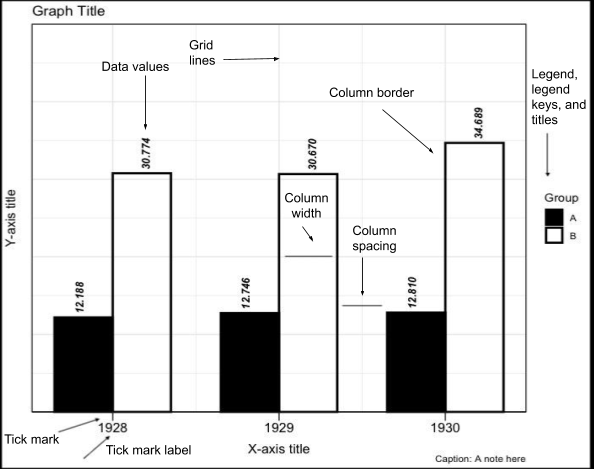
\includegraphics[width=12cm,height=14cm,keepaspectratio]{deneme2.png}
	\captionof{figure}{An anatomy of a column bar graph.}
	\label{fig:mylabelfanatomy}
\end{figure}


\section{Column bar graphics used in this study}
\label{sec:graphs}

Due to World War I (1914-1918) and then Independence War (1919-1922), the country, which was founded in 1923, had to simultaneously deal with many infectious diseases such as smallpox, malaria, plague, syphilis, trachoma, tuberculosis, leprosy, and typhus. Due to the increasing number of infectious diseases and infected people, the government had to develop new public health policies and offer health care services through launching new hospitals, training health care workers (including medical doctors, nurses and so on), and producing disease diagnostic kits, drugs, serum, and vaccines. In spite of many impossibilities, the government had achieved great success in prevention of infectious diseases during the period of 1923-1937. In 1938, all the efforts, especially the ones on the workload of hospitals and then on vaccine administration in the country, were summarized officially and these official statistics were visualized through statistical column bar graphics along with the tabular raw data in the government report. We should note that the government report does not provide any additional information or explanation related to these graphics. 

In this study, among these historical column bar graphics, we investigated and reproduced nine of them. We provide the original graphics alongside the reproduced graphics as well. In this sense, we categorize them into five main parts with respect to the number of data series available as well as grouping structure  of the bars (e.g., overlapped, side-by-side, and paired bar graphs). We also kindly invite readers to look at the \code{R} codes available as a Supplementary material while investigating the graphics.

\subsection{\textit{Bar graph with one data series}}

In the bar graphs with one data series, bars are used to compare a single numerical variable per item or category.  Figure~\ref{fig:mylabelf1org} gives the amount of smallpox vaccine administered in various regions of the country between the period $1925$ and $1937$. Smallpox is a deadly infectious disease accompanied by lesions filled with thick liquid appearing on the face, mouth, nose, and body of a person. Within the early days of exposure, it had been shown that the vaccination can prevent or lessen the severity of the disease. For that reason, the vaccination was mandatory for new borns, at schools, and at some workplaces. Note that these vaccines were distributed for free to prevent the disease.

In Figure~\ref{fig:mylabelf1org}, we can see that the background color of the figure is white. There is no vertical axis and related information on the vertical axis (e.g., axis line, axis title, axis tick marks, and tick mark labels). We can get the frequencies of each column bar through the data values placed inside the columns. Consequently, the column bar heights are directly proportional to the data values they represent. Since the height of the columns are taller and take space in the figure plotting area, the data values are placed vertically inside the columns. The horizontal axis refers to the time interval with linear increments without having an axis title.  Due to the white background color of the figure, the column bars are filled in with black color whereas the data values are colored in white for contrast. Due to a large number of column bars and lack of space, bar widths and the spacing between columns are kept short and the labels of the horizontal axis tick marks are displayed vertically. 

Since the heights of the columns of the graph are directly proportional to the data value they represent,  the \code{geom\_col()} layer right after the main \code{ggplot()} call in \pkg{ggplot2}  is used to produce Figure~\ref{fig:mylabelf1}. The data values are placed onto the graphic via an \code{annotate()} layer. The white background is obtained via \code{theme\_classic()} layer. 
The structure of the graph is mostly obtained  through modifying the components of \code{theme()} layer such as \code{axis.line}, \code{axis.title}, \code{axis.ticks}, and \code{axis.text} in \pkg{ggplot2},  in addition to \code{geom\_col()} layer. The main figure title consists of four lines. However, the first three line and the last line of the title have different font types, sizes, and  faces (i.e., italic and unitalic texts).  For that reason, several \code{annotate()} layers are further used to run the full title rather than \code{ggtitle()} or \code{labs()} layer which assumes a uniform text structure over the multiple lines. Finally, we can see that the number of smallpox vaccines administered increased over the years.

\begin{figure}[ht!]
	\centering
	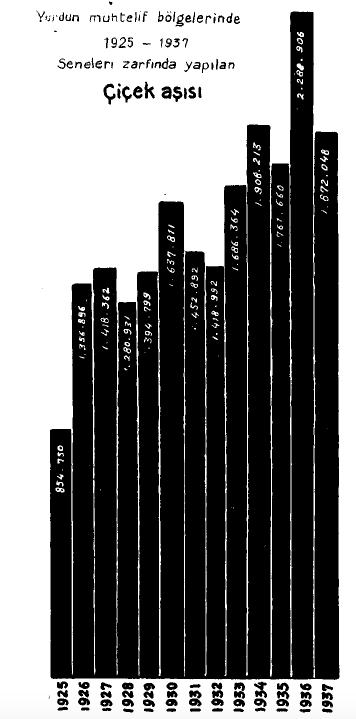
\includegraphics[width=9cm,height=12cm,keepaspectratio]{Cicek_original.png}
	\captionof{figure}{Historical figure on "Smallpox vaccine administered in various regions of the country, between the period 1925-1937" retrieved from \url{https://acikerisim.tbmm.gov.tr/handle/11543/553}.}
	\label{fig:mylabelf1org}
\end{figure}

%keepaspectratio
\begin{figure}[ht!]
	\centering
	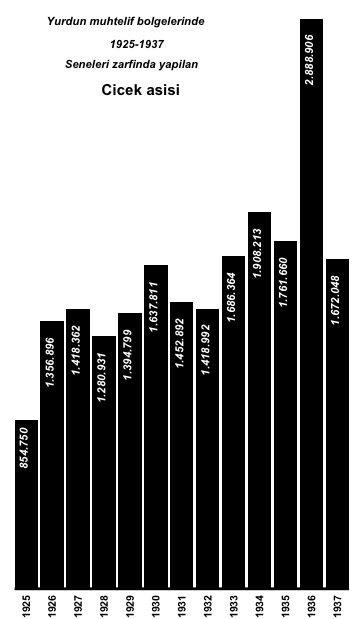
\includegraphics[width=7cm,height=14cm,keepaspectratio]{Cicekrep2.png}
	\captionof{figure}{Reproduced figure on "Smallpox vaccine administered in various regions of the country, between the period 1925-1937".}
	\label{fig:mylabelf1}
\end{figure}


\subsection{\textit{Overlapped bar graphs with two data series}}

\begin{figure}[ht]
	\centering
	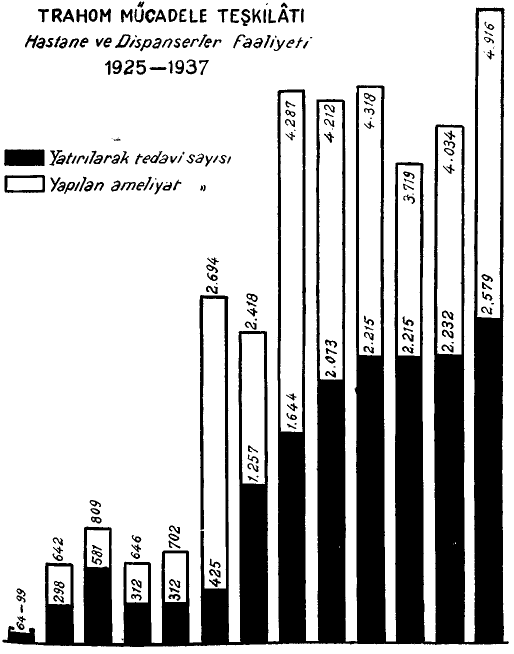
\includegraphics[width=12cm,height=11cm,keepaspectratio]{Trahom_original.png}
	\captionof{figure}{\label{fig:mylabelf3org} Historical figure on "The service of hospitals and dispensaries within the Department of Control of Trachoma, 1925-1937" retrieved from \url{https://acikerisim.tbmm.gov.tr/handle/11543/553} ($\blacksquare$ The number of inpatient treatments $\square$ The number of surgeries performed).}
\end{figure}


\begin{figure}[ht!]
	\centering
	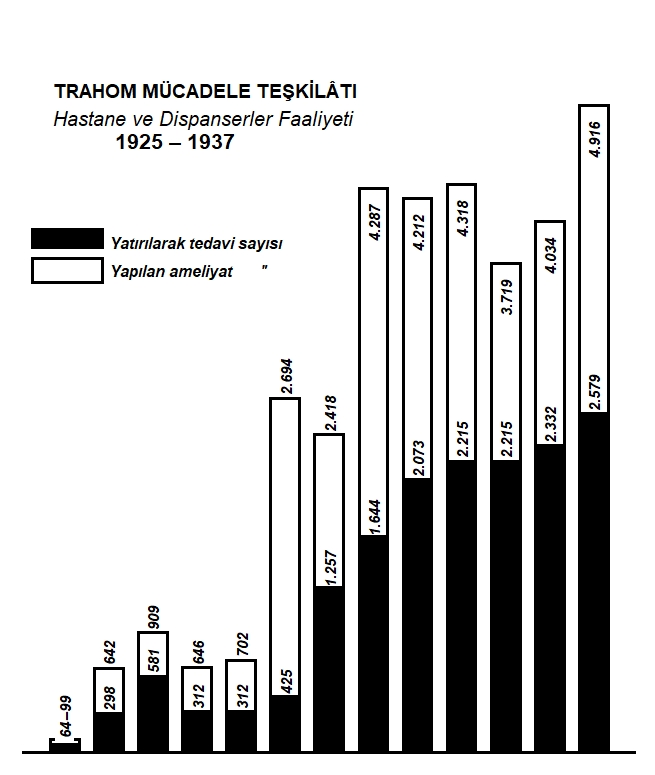
\includegraphics[width=12cm,height=12cm,keepaspectratio]{Trahomrep.png}
	\captionof{figure}{\label{fig:mylabelf3} Reproduced figure on "The service of hospitals and dispensaries within the Department of Control of Trachoma, 1925-1937" ($\blacksquare$ The number of inpatient treatments $\square$ The number of surgeries performed).}
\end{figure}


Figure~\ref{fig:mylabelf3org} presents the service of hospitals and dispensaries within the Department of  Control of Trachoma between the years $1925$ and $1937$ with respect to the number of inpatient treatments performed (in black) and the number of surgeries performed for treating trachoma (in white).

Trachoma is an infectious eye disease caused by a bacteria and is transmitted among humans through shared use of items used for cleaning face. If it is not treated at the earlier stages, it may lead to damages in eye cornea or even to blindness. In the early stages of trachoma, antibiotics may be effective to eliminate the infection, whereas surgery may be required at the later stages.

As in Figure~\ref{fig:mylabelf1org}, the background color of the Figure~\ref{fig:mylabelf3org} is white and there is no vertical axis and any information related to the vertical axis (e.g., axis line, axis title, axis tick marks, and tick mark labels). The columns of both groups are overlapped $100\%$ and the column bar heights are directly proportional to the data values they represent. 
The data set for the number of inpatient treatments is always shorter than the data set for the number of surgeries performed for treating trachoma over the years $1925$ and $1937$. Thus, the columns for inpatient treatments are positioned in front of the columns for the number of surgeries performed.  However, the disparity between the heights of both groups is manipulated through assigning a strong color, black, to the number of inpatient treatments, and a recessive color, white, to the number of outpatient treatments, which is a common strategy in graphic design \citep{White}. This emphasis is also reflected in the legend keys such that the legend keys are ordered according to color, not alphabetically. 

The data values for the surgery group between the years $1925$ and $1931$ are placed vertically at the top of the columns. Those between the years $1932$ and $1937$ are placed inside the columns vertically due to lack of space in the plotting region, whereas the data values for the number of inpatient treatments are always placed vertically inside the column.  All the  data values for each group are in black since the background color is white. Due to the reasonable number of column bars in the plotting area, the width of the column bars and the inter-bar spacing between them are now increased.

Unlike Figure~\ref{fig:mylabelf1org}, there are no labels for the horizontal axis tick marks now. However, the third line of main graph title gives the clue that horizontal axis starts from $1925$ and goes to $1937$.  As the reviewer pointed out, we think that horizontal tick mark labels here were unintentionally forgotten since this is the only bar graph with missing horizontal tick mark labels in the government report. However, this may result in a cognitive effort for the viewer if the viewer would like to know the exact information for the number of inpatient treatments and/or the number of surgeries performed throughout the years, especially for the years in the middle of 1925 and 1937. In that case, the viewer has to count the number of bars to get precise information. On the other hand, if the interest is on the overall trend of the number of inpatient treatments and/or the number of surgeries performed over the years, then  comparing the heights of the bars visually will eliminate this problem. If there is not enough space to place all the tick marks on the horizontal axis, then two design choices can be followed here: 1) placing all the labels with some vertical shift such as 90 degree or 45 degree alignment, or 2) starting labeling at the year 1925 and labeling the years with one year apart.
	 	 
In Figure~\ref{fig:mylabelf3}, the $100\%$ overlapping structure of column bars is obtained via setting argument \code{position = "identity"} in \code{geom\_col()} layer. Note that the look of Figure~\ref{fig:mylabelf3} requires arrangement of the levels of grouping factor in the data with order of inpatient treatments and surgeries performed, respectively. This grouping variable  is also mapped into  \code{fill}  and   \code{alpha}  arguments of the aesthetics of the main \code{ggplot()} call 
since the fill-in colors of the bars and transparency level of the bars should be matched with the levels of this grouping variable. In addition to modifying several components of \code{theme()} layer,  assigning \enquote{black} color to the inpatient treatments and \enquote{white} color to the surgeries performed via \code{scale\_fill\_manual()} layer, and then assigning low level of transparency \enquote{1} to the black color of inpatient treatments and high level of transparency \enquote{0} to the white color of surgeries performed via \code{scale\_alpha\_manual()} layer would yield the final look of the figure. Hence, the order of elements of the vector of colors in \code{scale\_fill\_manual()} layer and the order of elements of the vector of transparency in \code{scale\_alpha\_manual()} layer are matched with the order of the levels of the grouping variable. Lastly, if  transparency were not added to the plot, the color of the second level of the grouping variable will be displayed only due to the overlapping structure of the column bars.

The white line segment in the first column of Figure~\ref{fig:mylabelf3} is integrated via an \code{annotate()} layer along with \code{rect} argument. On the other hand, three-lined main graph title is run with \code{labs()} and \code{annotate()} layers due the italicized font structure of the middle line compared to the unitalicized font structure of the first and the last lines. Lastly, we can say that both the number of inpatient treatments and the number of surgeries performed increased considerably over the years.

Figure~\ref{fig:mylabelf4org} shows the service of the Zonguldak Government Hospital between the years $1924$ and $1937$ with respect to the number of inpatient treatments (in black) and the number of outpatient treatments (in white). The data value for the number of outpatient treatment is not available in $1924$ and is coded as \strong{NA} in the data. While the columns for the number of inpatient treatments are taller than that of outpatient treatment over the period $1925$ and $1932$, the columns for the number of outpatient treatments are taller than that of inpatient treatments over the period $1933$ and $1937$. To increase the dominance of the number of inpatient treatments over the number of outpatient treatments, the former group is colored in black.

\begin{figure}[hbt!]
	\centering
	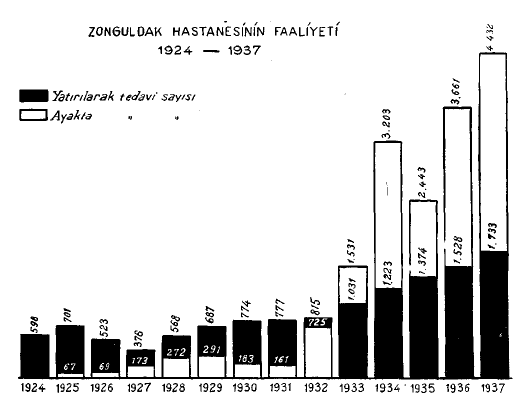
\includegraphics[width=12cm,height=12cm,keepaspectratio]{Zonguldak_original.png}
	\captionof{figure}{\label{fig:mylabelf4org} Historical figure on "The service of the Zonguldak Government Hospital, 1924-1937" retrieved from \url{https://acikerisim.tbmm.gov.tr/handle/11543/553} ($\blacksquare$ The number of inpatient treatments  $\square$ The number of outpatient treatments).}
\end{figure}

\begin{figure}[hbt!]
	\centering
	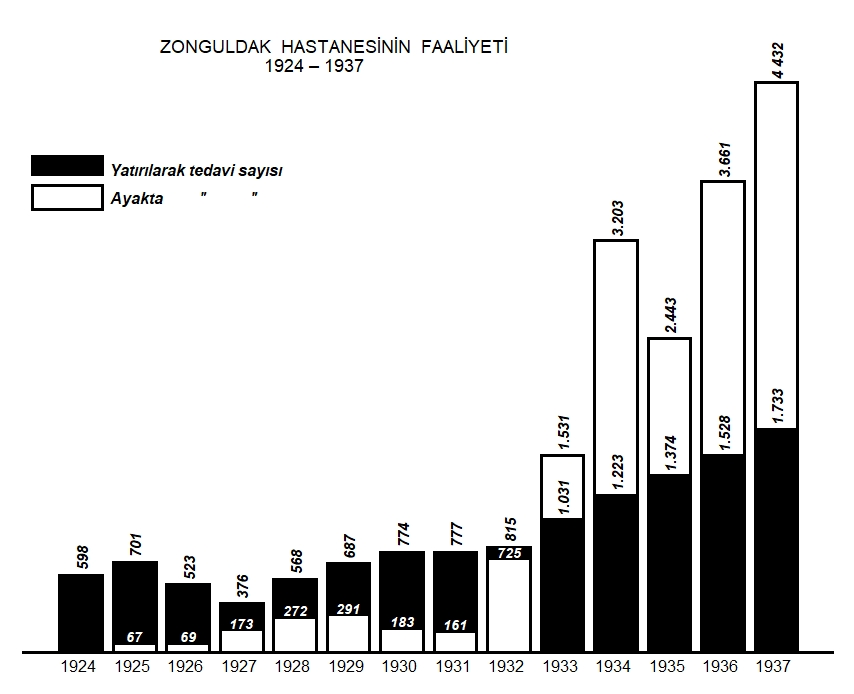
\includegraphics[width=12cm,height=12cm,keepaspectratio]{Zonguldakrep.png}
	\captionof{figure}{\label{fig:mylabelf4} Reproduced figure on "The service of the Zonguldak Government Hospital, 1924-1937"  \linebreak ($\blacksquare$ The number of inpatient treatments  $\square$ The number of outpatient treatments).}
\end{figure}

In year 1932, the number of outpatient treatments is close to the number of inpatient treatments in magnitude, where the frequencies are 725 and 815 respectively. Since there is not enough space to place the number 725 vertically inside the bars, it is aligned horizontally and colored in white due to the black background color. To be consistent with white front-positioned outpatient treatment bars,  
all the data labels of outpatient treatments are placed horizontally between $1925$ to $1932$ and then vertically onwards. This approach gives a practical information design approach.

The \code{R} code structure of  Figure~\ref{fig:mylabelf4} is very challenging and is not straightforward since  \code{geom\_col(posi\linebreak tion = "identity")} assumes that difference between two data series over the years takes a uniform behaviour, i.e., it assumes that a series is always either greater than the other one, or always less than the other one. If  it is not so, \code{geom\_col(position  = "identity")},  \code{scale\_fill\_manual()}, and \code{scale\_alpha\_manual()} layers cannot handle the zig-zag pattern in the difference of data series when drawing bars. This problem actually opens a research door for \pkg{ggplot2}. 

Figure~\ref{fig:mylabelf5org} represents the workload of private hospitals between the years $1926$ and $1937$ with respect to the number of inpatient treatments (in black) and the number of outpatient treatments (in white). Except the year $1926$, the columns for the number of inpatient treatments are always shorter than the columns for the number of outpatient treatments. In $1926$, the number of inpatient treatments is $17,700$, which is greater then the number of outpatient treatments, $16,009$. The columns, which are positioned in the front, are shifted to the left, resulting in around $70\%$ overlapping. Due their front position and stronger color, the number of inpatient treatments take the attention of the viewer. On the other hand, since the data values for the number of outpatient treatments is just twice of the data values for the number of inpatient treatments in the years $1927$ and $1928$, the heights of the column bars are close to each other and hence there is not enough space to place the data values for the number of inpatient treatments in the column bars vertically. To avoid overlapping of  two data labels, the front data labels are placed horizontally, which is a practical approach. 
This information gives us an another idea that alignment of data values according to space available in Figures~\ref{fig:mylabelf4org} and ~\ref{fig:mylabelf5org} is reasonable. However, as the reviewer pointed out, this inconsistencies i.e., aligning texts horizontally then vertically,  is visually distracting and may decrease the readability. 


\begin{figure}[hbt!]
	\centering
	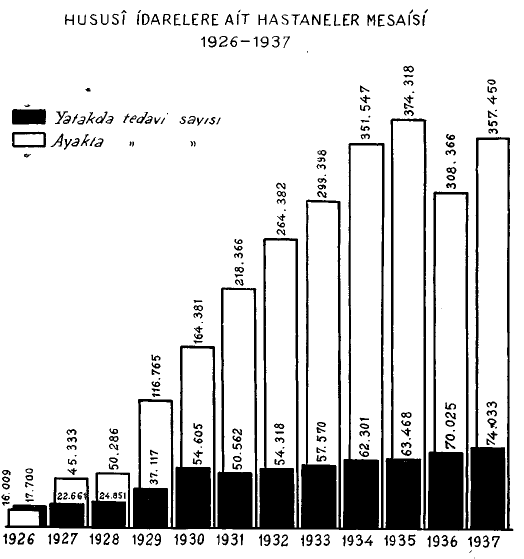
\includegraphics[width=12cm,height=11cm,keepaspectratio]{Hususi_original.png}
	\captionof{figure}{\label{fig:mylabelf5org} Historical figure on "The workload of private hospitals, 1926-1937" retrieved from \url{https://acikerisim.tbmm.gov.tr/handle/11543/553} ($\blacksquare$ The number of inpatient treatments  \linebreak $\square$ The number of outpatient treatments).}
\end{figure}


\begin{figure}[hbt!]
	\centering
	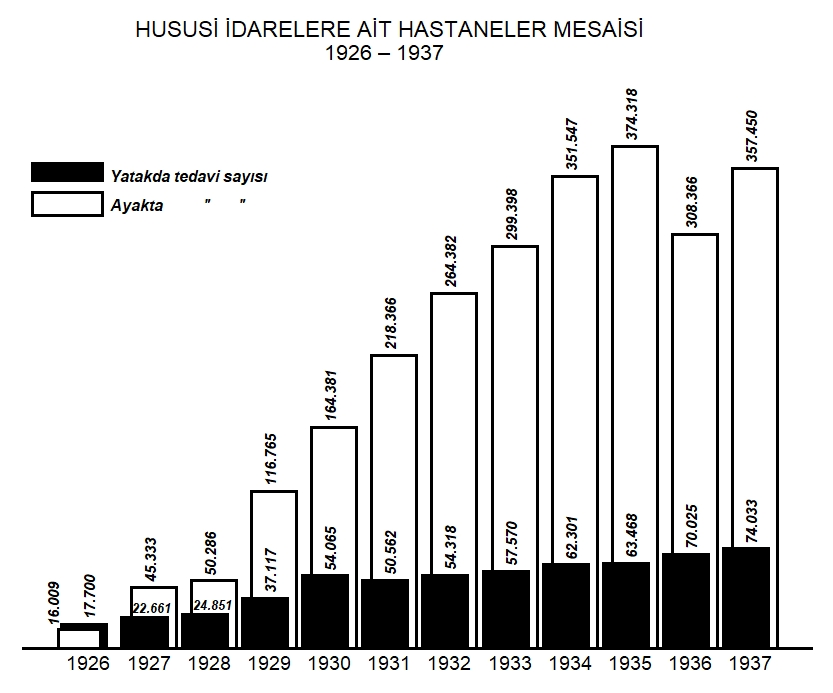
\includegraphics[width=12cm,height=12cm,keepaspectratio]{Hususirep.png}
	\captionof{figure}{\label{fig:mylabelf5} Reproduced figure on "The workload of private hospitals, 1926-1937" ($\blacksquare$ The number of inpatient treatments $\square$ The number of outpatient treatments).}
\end{figure}


The \code{R} code structures of Figures~\ref{fig:mylabelf3} and \ref{fig:mylabelf5} are very similar to each other. The $70\%$ overlapping position of columns bars in Figure~\ref{fig:mylabelf5} is adjusted through setting 
\code{position = position\_dodge(width = 0.3)} in \code{geom\_col()} layer.
Furthermore, in year 1926, the column of outpatient treatment is less than that of inpatient treatment, which is vice versa in the subsequent bars. As we discussed a similar problem for Figure~\ref{fig:mylabelf4},  \code{geom\_col(position = "identity")} could not handle this and the white rectangular column bar in year 1926 is drawn manually via \code{annotate()} layer  with \code{rect} argument. 
	
In Figures~\ref{fig:mylabelf3org}, \ref{fig:mylabelf4org}, and \ref{fig:mylabelf5org}, the legend is placed vertically at the top-left of the plotting area, since the overall structure of the graphs are left-skewed and the legend keys are ordered according to color, not alphabetically. Furthermore, in Figures~\ref{fig:mylabelf3org}-\ref{fig:mylabelf5}, the double apostrophe, " , in the title of second legend key is  a typographic symbol, called  a ditto mark, which is used for repeated words above it. In hand-written texts, ditto mark is used to save time and effort from the writer. Since the government report includes around forty figures, this may be the reason why ditto mark is also used in the legend key titles. While this approach also reduces the amount of ink used in the figures, it does not distort the readability of the graph. However, we should note that in today's technology, the repetitive words can be typed as needed with less effort.

We would like to note that the Figures~\ref{fig:mylabelf3org}, \ref{fig:mylabelf4org}, and \ref{fig:mylabelf5org} may look like as if they were stacked bar graphs. However, since the government report published in $1938$ includes the raw tabular data in it, we are $100\%$ confident to say that these figures are overlapped bar graphs. Furthermore, we would also like to note that in stacked bar charts, the height of the column bar gives the total frequency of all groups on a given year. If one needs the frequency of a specific group on that year, then an additional arithmetic operation such as subtraction should be done to calculate it. Keeping in mind that these graphs are presented to the public who has a low level of literacy, doing an extra mathematical work in stacked bar charts would add a computational burden to the viewer, which may not be possible for the viewer at that time.

Another distinction between overlapped bar graphs and stacked bar graphs is that overlapped bar graphs are used to display the comparison between two closely related numerical variables over an item/category (here it is years), whereas stacked bar graphs are used to display comparison at least two complementary numerical variables over an item/category. As we can see from the Figures~\ref{fig:mylabelf3org}, \ref{fig:mylabelf4org}, and \ref{fig:mylabelf5org}, the variables of interests, which are inpatient vs outpatient or inpatient vs surgeries performed, are closely related to each other, not directly mutually exclusive events. Furthermore, the offset (dodging) in the Figure~\ref{fig:mylabelf5org} also confirms that columns are overlapped.

Lastly, the increasing trends in the number of inpatient treatments  in Figures~\ref{fig:mylabelf4org} and \ref{fig:mylabelf5org} may indicate that the hospital bed capacity increased over the years, whereas a stabile trend shows that the hospital's bed capacity did not change over the years. On the other hand, increasing trends in the number of outpatient treatments may indicate an increase in general service capacity of the hospital.

\subsection{\textit{Grouped side-by-side bar graphs with two data series}}

Figure~\ref{fig:mylabelf6org} represents the workload of sample hospitals between the years $1924$ and $1937$. There are also two groups here: inpatient and outpatient treatments, colored in black and white respectively. Figure~\ref{fig:mylabelf6org} is different from previous ones since the columns for inpatient and outpatient treatments for the same year are now placed side-by-side accordingly. This can be done by setting the argument \code{position = position\_dodge2()} in the \code{geom\_col()} layer.  The grouping variable is mapped into \code{fill} argument of the aesthetics of the main \code{ggplot()} call so that color of the levels of the grouping variable can be assigned manullay  in \code{scale\_fill\_manual()} layer.

There is only one column in the year $1924$ because there is no information available for the outpatient treatment in $1924$. It is coded as \strong{NA} in the data.  The length of the column bars for the number of inpatient treatments are shorter than those of the outpatient treatments over the years. However, to increase the dominance of the number of inpatient treatments over the number of outpatient treatments, the inpatient treatment group is colored in black and placed ahead of outpatient treatment group, an information design stragety which we learned from \cite {White}. The data values for both groups are placed at the top of columns vertically due to enough space in the plotting area. 

The Figures~\ref{fig:mylabelf4org} and ~\ref{fig:mylabelf6org}
are good examples  that \code{geom\_col()} layer in \pkg{ggplot2} can handle missing values in the data. In other words \pkg{ggplot2}can handle unequal length of data series for a given category (here it refers to a given year) while sketching  overlapped and side-by-side bar graphs. On the other hand, a literature survey revealed that the Zonguldak Government Hospital in the Figure~\ref{fig:mylabelf4org} and the sample hospitals in the Figure~\ref{fig:mylabelf6org} were launched in 1924 as the second-stage hospitals in the cities offering inpatient services with specialized health workers such as doctors, nurses,  and laboratory services. In the cities where these hospitals were available, a person with medical complications  was initially admitted to the small hospitals with low health care capacity as the first-stage hospitals, and only the ones who needed inpatient services in a specialized medical area were transferred to the second-stage hospitals. For that reason, there is no data value for outpatient treatments in the Figures~\ref{fig:mylabelf4org} and \ref{fig:mylabelf6org} in 1924. After 1924, due to on-going efforts improving health care policies and hospital capacities, these main hospitals started to offer both outpatient and inpatient treatments.


\begin{figure}[hbt!]
	\centering
	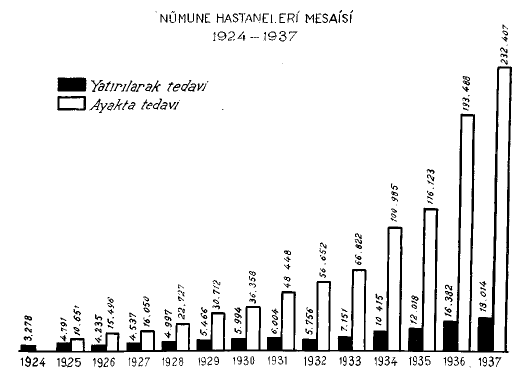
\includegraphics[width=12cm,height=12cm,keepaspectratio]{Numune_original.png}
	\captionof{figure}{\label{fig:mylabelf6org} Historical figure on "The workload of sample hospitals, 1924-1937" retrieved from \url{https://acikerisim.tbmm.gov.tr/handle/11543/553} ($\blacksquare$ Inpatient treatment $\square$ Outpatient \linebreak treatment).}
\end{figure}

\begin{figure}[hbt!]
	\centering
	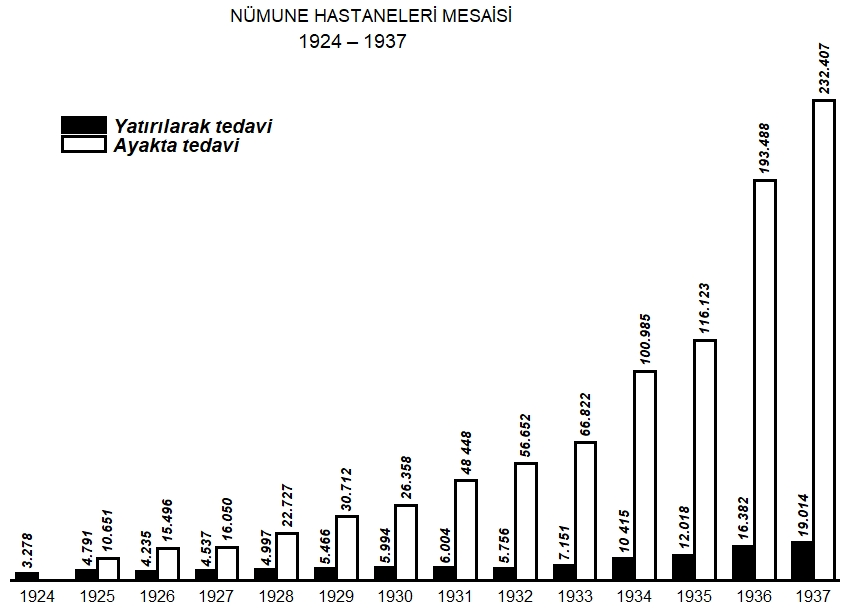
\includegraphics[width=12cm,height=12cm,keepaspectratio]{Numunerep.png}
	\captionof{figure}{\label{fig:mylabelf6} Reproduced figure on "The workload of sample hospitals, 1924-1937" ($\blacksquare$ Inpatient treatment $\square$ Outpatient  treatment).}
\end{figure}

Figure~\ref{fig:mylabelf7org} represents the laboratory workload for Malaria struggle between the years $1925$ and $1937$. The white color refers to the number of blood tests performed and the black color refers to the number of diagnoses. As in Figure~\ref{fig:mylabelf6org}, in Figure~\ref{fig:mylabelf7org}, the paired columns for the same year are now placed side-by-side. The columns for the number of blood tests are taller than the columns for the number of diagnoses over the years $1925$ and $1937$. Placing the number of blood tests ahead of the number of diagnoses enables us to compare how many blood tests resulted in a positive Malaria diagnosis (like today, the world is now comparing \enquote{the number of Covid-19 tests performed} with \enquote{the number of positive test results}). Although the number of diagnoses is smaller, coloring it in black increased its importance and softened the disparity between the sizes of the pair, which is an information design principle given in \cite{White}. Since the number of diagnoses falls behind the number of blood tests, vertically placing the horizontal axis tick mark labels in black color makes an illusion and increases the dominance of the number of diagnoses (in black) in the graphic. 


\begin{figure}[hbt!]
	\centering
	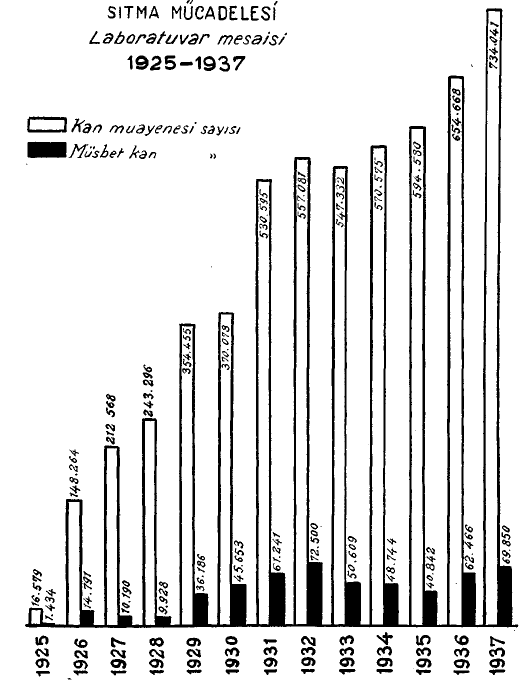
\includegraphics[width=15cm,height=11cm,keepaspectratio]{Sitma_original.png}
	\captionof{figure}{\label{fig:mylabelf7org} Historical figure on "The laboratory workload for Malaria struggle, 1925-1937" retrieved from \url{https://acikerisim.tbmm.gov.tr/handle/11543/553} ($\square$ The number of blood tests \linebreak $\blacksquare$ The number of diagnoses).}
\end{figure}


\begin{figure}[hbt!]
	\centering
	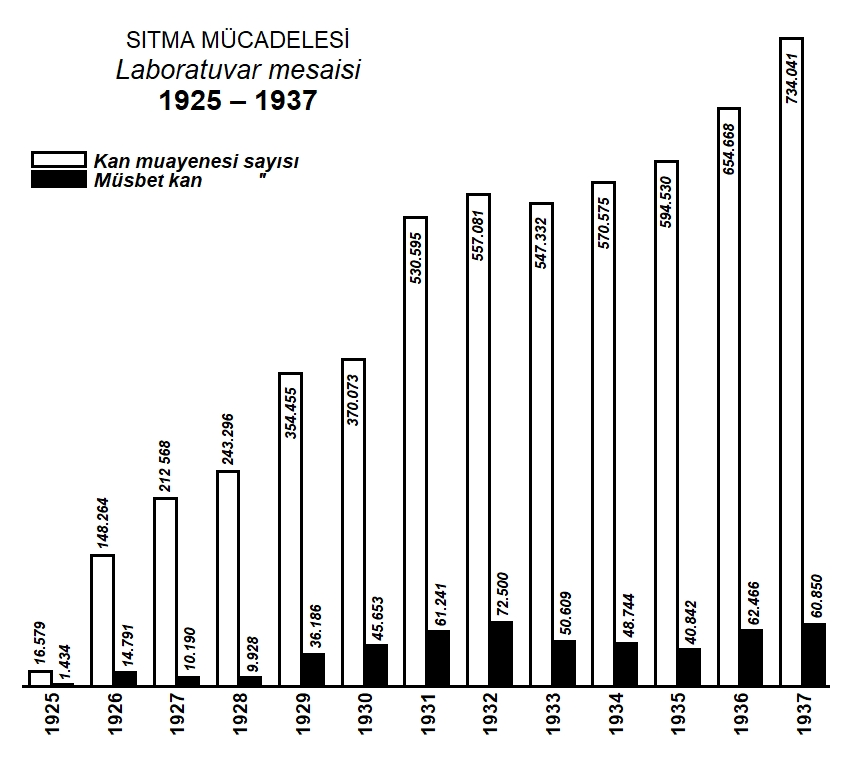
\includegraphics[width=10cm,height=12cm,keepaspectratio]{Sitmarep.png}
	\captionof{figure}{\label{fig:mylabelf7} Reproduced figure on "The laboratory workload for Malaria struggle, 1925-1937" ($\square$ The number of blood tests $\blacksquare$ The number of diagnoses).}
\end{figure}


The data values for the number of diagnoses are easily placed at the top of columns vertically due the shorter length of corresponding columns. However, while the data values for the number of blood tests are placed at the top of the column vertically between the years $1925$ and $1928$, the data values for the number of blood tests between the years $1929$ and $1935$ are placed inside the column bars vertically due to the space limitation in the plotting region. 

In the Figures~\ref{fig:mylabelf6org} and \ref{fig:mylabelf7org},  the space between groups of bars is increased and now equals to the width of a single bar in a given group. On the other hand, space between bars within a group is not available. 

The legends in the Figures~\ref{fig:mylabelf6org} and \ref{fig:mylabelf7org} are placed vertically at the top-left of the figures since the overall structure of graphs are left-skewed. 
Note that the ordering in the group colors are also reflected in the legend keys as well. For example, in Figure~\ref{fig:mylabelf7org}, the first legend is in white and the second one is in black. Here we note that in the Figures~\ref{fig:mylabelf6} and \ref{fig:mylabelf7}, the legend key order is inherited from the order of the level of the grouping variable in each plot and this grouping variable is declared in \code{fill} argument of the aesthetics of the main \code{ggplot()} call. The color of the legend keys are also matched with the color of the corresponding level of the grouping variable which was assigned in \code{scale\_fill\_manual} layer(). Lastly, from Figures~\ref{fig:mylabelf7org}, we can say that the government kept administrating blood tests over the years with an increasing trend and nearly $10\%$ of them were being turned out to be positive. 


\subsection{\textit{Grouped side-by-side bar graph with more than two data series}}

Figure~\ref{fig:mylabelf12org} represents the drugs sent by the Department of Control of Syphilis to cities for treatment between the period $1926$ and $1937$. Syphilis is a sexually transmitted disease caused by a bacteria and it has bee a very serious public health problem in the world since $1800$'s. Several antibiotic-based drugs were used to cure the Syphilis.

In the Figure~\ref{fig:mylabelf12org} we can see that there are four different drug types: Arsenobenzol, Bizmopen, Mercury, and Iodine, where they are filled in with black color, white color, textured with vertical lines, and textured with dots, respectively. This textured design is specifically called hatching in graphic design. 

To emphasize grouping over the years, the horizontal axis is broken into segments. It can also be seen from the figure that there were Bizmopen and Mercury drugs in $1926$ only; there were Arsenobenzol, Bizmopen, and Mercury drugs between the years $1927$ and $1933$, and afterwards, the fourth drug Iodine came out in $1934$. Regardless of the number of drugs available at a specific year, the width of grouping is always kept uniform over the years $1926$ and $1937$. 

The data series for the groups are placed side-by-side, which can be done by setting argument \code{position = position\_dodge()} in the \code{geom\_col()} layer. The order in the placement of the groups is also reflected in the legend keys. A side note is also attached to the graph telling that \enquote{The counts show kilo}. Adding captions to the graphs is possible via \code{caption} argument in \code{labs()} layer of \pkg{ggplot2}. 

On the other hand, we should say that some of  the raw materials of these four drugs were imported from abroad, the treatment of  syphilis was mandatory and free. Similarly, these four drugs were distributed free to the patients. In the Figure~\ref{fig:mylabelf12org} the columns for the Mercury filled with vertical lines are very eye-catching due to their taller heights. While \citet{Si} says that Mercury had been commonly used to cure Syphilis  until discovery of penicillin around $1940$'s ,   \citet{mumyakmaz7illet} reported that the mercury was the most effective drug to treat the patients ($95\% $ effective), and the Iodine was the second effective drug.

The Figure~\ref{fig:mylabelf12org} is a good example for use of hatching for differentiating the data groups when there is no color option or color printing was not easy or economical in 1938.  However, this resulted in a challange that textured patterns are not allowed in the core functions of the \pkg{ggplot2} package. For that reason, we used several \code{annotate()} layers along with \code{segment} argument to integrate hatches with vertical lines and dots into the column bars. Since we did hatching manually, we could not synchronize textured patterns in the column bars with the legend keys. As a consequence of this, several \code{annotate()} layers with \code{rect} argument for drawing the legend boxes, several \code{annotate()} layers with \code{segment} argument for filling the textured patterns in legend keys, and several \code{annotate()} layers with \code{text} argument for typing the legend key titles were used. 

We also provided three different historical column bar graphics along with \code{R} codes in the Supplementary material for further interest.

\begin{figure}[hbt!]
	\centering
	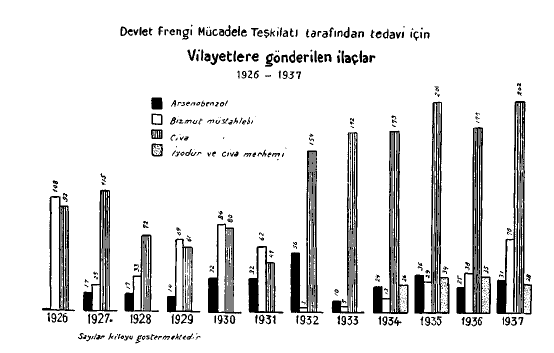
\includegraphics[width=13cm,height=18cm,keepaspectratio]{Frengi_original.png}
	\captionof{figure}{\label{fig:mylabelf12org} Historical figure on "The drugs sent by the Department of Control of Syphilis to cities for treatment, 1926-1937" retrieved from \url{https://acikerisim.tbmm.gov.tr/handle/11543/553} ($\blacksquare$ Arsenobenzol  $\square$ Bizmopen  \crule[gray]{0.30cm}{0.30cm} (textured pattern with vertical lines)  Mercury \legendsquare{pattern=dots}~Iodine).}
\end{figure}

\begin{figure}[hbt!]
	\centering
	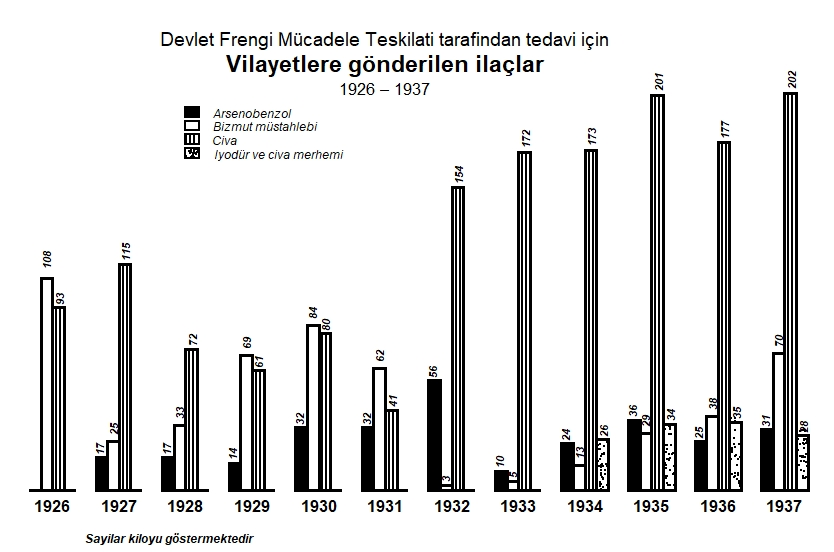
\includegraphics[width=12cm,height=14cm,keepaspectratio]{Frengirep.png}
	\captionof{figure}{\label{fig:mylabelf12} Reproduced figure on "The drugs sent by the Department of Control of Syphilis to cities for treatment, 1926-1937" ($\blacksquare$ Arsenobenzol  $\square$ Bizmopen  \crule[gray]{0.30cm}{0.30cm} (textured pattern with vertical lines)   Mercury \legendsquare{pattern=dots}~Iodine).}
\end{figure}


\subsection{\textit{Paired bar graphs with two data series}} 

Figure~\ref{fig:mylabelf13org} shows the total number of serums and vaccines, which are produced and consigned, at the Central Hygiene Institute for the years between $1930$ and $1937$. The Central Hygiene Institute was a reference laboratory in the country launched for producing serum and vaccine for several infectious diseases such as rabies, typhoid, and whooping cough. 

Figure~\ref{fig:mylabelf13org} breaks down the data into two panels as produced (left-panel) and cosigned (right-panel) through a vertical axis. The left side of vertical axis is for the number of produced serum and  vaccine items in kilogram and the right side of the vertical axis is for the number of consigned serum and vaccine items in kilogram. Under each panel, the data set for serum (in black) and vaccine (in white) are displayed via overlapping columns from $1930$ to $1937$. The legend keys for serum (in black) and vaccine (in white) are separated horizontally. Note that this is the first time a vertical axis appears in a graph and it is placed at the center of the graph. It denotes the years with the title \enquote{Yillar} and descends from $1937$ to $1930$. Since the columns of recent years are taller than the columns of earlier years, which also shows the continuing success of the institute, reversing the order of years (starting from the recent year $1937$) makes the graphic to look like a population pyramid. Furthermore, although data values are annotated to the column bars, a horizontal axis with tick marks and tick mark labels are also available. The tick mark labels show the respective counts, which are not linear in magnitude, going from $0$ to $4500$ with unequal increments. The horizontal axis title \enquote{SAYISI} refers to the \enquote{Frequency}. This is the first time we have a horizontal axis title as well. The text aligned with 45 degree at the left panels refers to the \enquote{PRODUCED (IN KILO)} and the one with 135 degree at the right refers to the \enquote{CONSIGNED IN (KILO)}, which are symmetric to each other with respect to the vertical axis. We can consider this graph as a paired bar graph having a double horizontal axis with a common vertical axis.  Lastly, here we can see that the country was very successful both at producing and consigning vaccine in 1930's due to increasing trend over the years.

\begin{figure}[hbt!]
	\centering
	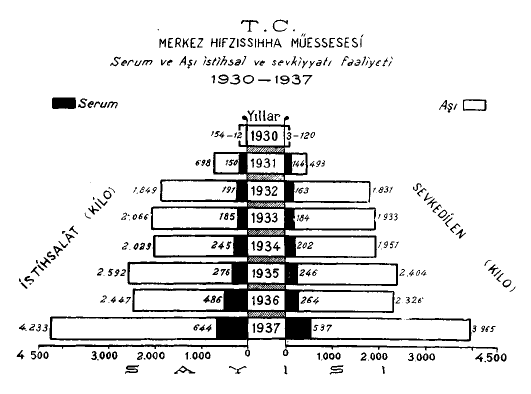
\includegraphics[width=12cm,height=19cm,width=9cm,keepaspectratio]{Serum_original.png}
	\captionof{figure}{\label{fig:mylabelf13org} Historical figure on "The service of produced and consigned serum and vaccine in kilogram at the Central Hygiene Institute, 1930-1937" retrieved from \url{https://acikerisim.tbmm.gov.tr/handle/11543/553} (The left-panel is for produced items and the right-panel is for consigned times; $\blacksquare$ Serum $\square$ Vaccine).}
\end{figure}


\begin{figure}[hbt!]
	\centering
	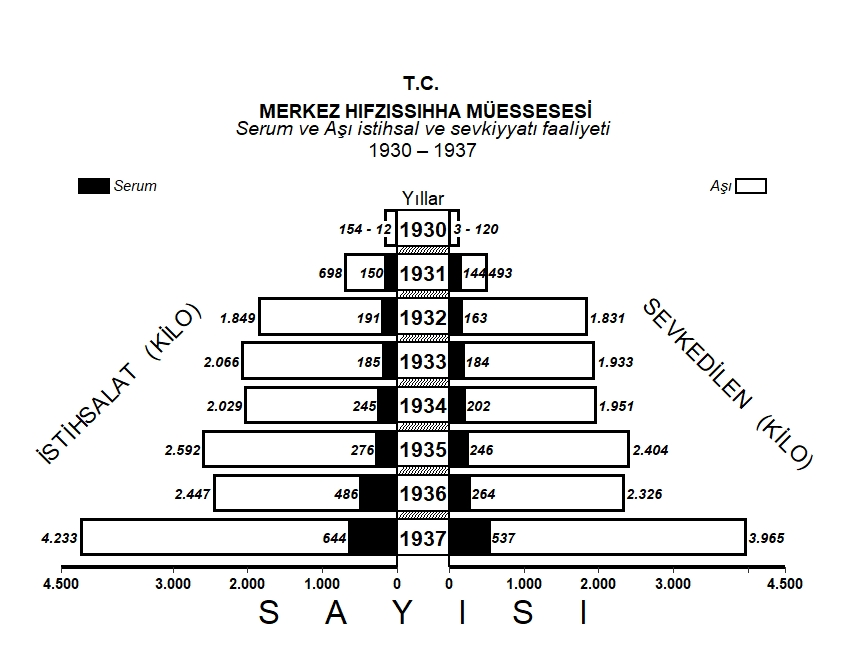
\includegraphics[width=12cm,height=19cm,width=9cm,keepaspectratio]{Serumrep.png}
	\captionof{figure}{\label{fig:mylabelf13} Reproduced figure on "The service of produced and consigned serum and vaccine in kilogram at the Central Hygiene Institute, 1930-1937" (The left-panel is for produced items and the right-panel is for consigned times; $\blacksquare$ Serum $\square$ Vaccine).}
\end{figure}

\begin{figure}[hbt!]
	\centering
	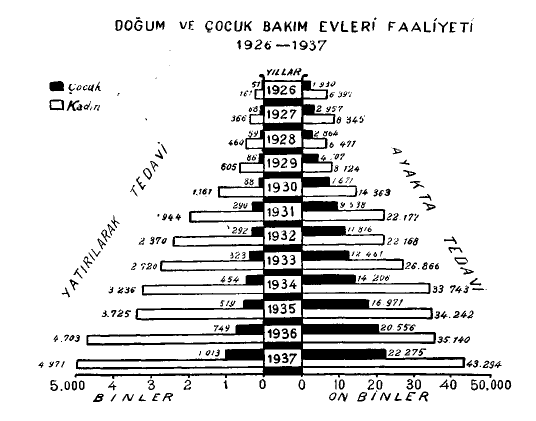
\includegraphics[width=12cm,height=14cm,keepaspectratio]{Dogum_original.png}
	\captionof{figure}{\label{fig:mylabelf14org} Historical figure on "The service of birth and childcare houses, 1926-1937" retrieved from \url{https://acikerisim.tbmm.gov.tr/handle/11543/553} (The left-panel is for inpatient services and the right-panel is for outpatient services; $\blacksquare$ Child $\square$ Woman).}
\end{figure}

\begin{figure}[hbt!]
	\centering
	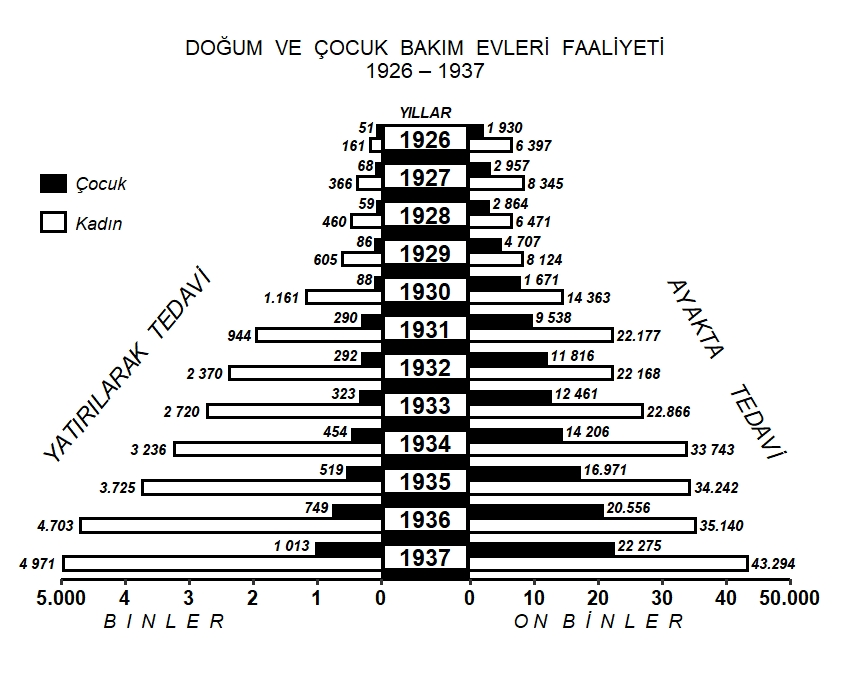
\includegraphics[width=12cm,height=12cm,keepaspectratio]{Dogumrep.png}
	\captionof{figure}{\label{fig:mylabelf14} Reproduced figure on "The service of birth and childcare houses, 1926-1937" (The left-panel is for inpatient services and the right-panel is for outpatient services; $\blacksquare$ Child $\square$ Woman).}
\end{figure}

Due to high infant mortality rates in the early years of the country, special effort was devetod the health care of mother and child.
Figure~\ref{fig:mylabelf14org} shows the service of birth and childcare houses for women and children between the period $1926$ and $1937$. As in Figure~\ref{fig:mylabelf13org}, the vertical axis breaks down the data into two panels as inpatient services (left-panel) and outpatient services (right-panel). Then for each panel, the data set for child and woman are displayed over the years $1926$ and $1937$ as side-by-side column bars in black and white colors, respectively. As in Figure~\ref{fig:mylabelf13org}, 
the vertical axis at the center denotes years by \enquote{Yillar} starting from $1937$ and descending to $1926$. The tick marks on horizontal axis show the respective frequencies with linear increments. The tick mark labels at left side of the horizontal axis represents the numbers in terms of \enquote{Thousands}, going from $0$, then to $1$, $2$, $3$, $4$, and $5000$. Similarly, tick mark labels at the right side of the horizontal axis represents the numbers in terms of
\enquote{Ten Thousands}, going from $0$, then to $10$, $20$, $30$, $40$, and $50,000$. Due to space limitation on the horizontal axis, the last three digits of the numbers are not used, except the last numbers ($5,000$ at the left and $50,000$ at the right). This looks like a promising example for information design of displaying very large numbers on graphics when there is no space to integrate all the text into the plotting area. Integration of these tick mark labels is done via \code{labels} argument of \code{scale\_y\_continuous()} layer in \pkg{ggplot2}. The paired bar graphs in the Figures~\ref{fig:mylabelf13} and \ref{fig:mylabelf14} can be plotted
via using multiple \code{geom\_col()} layers with some extra aesthetic work in \pkg{ggplot2} package. Here we should note that to be able to assign a pyramid look to the graph, the data is visualized with an illusion since height of the left-panel bars are actually pretty much smaller than the ones at right-panel.
Lastly, we can say that the country was also succesful at taking care of childs and mothers with an increasing number of inpatient and outpatient services over the years.


\section{Redesign of historical bar graphics in modern era}
\label{sec:redesign}


The historical graphics given above enable us to investigate the trends of several numerical variables over time and make comparisons between these numerical variables  through column bar graphics.
We can also re-visualize these graphics with the help of modern data visualization principles and software technology to increase the readibility and effectiveness of the graphs  through increasing the data-ink ratio given below:

\begin{equation}
\label{key}
\nonumber
\text{Data-ink ratio} = 	\frac{\text{Ink used to describe the data}}{\text{Ink used to visualize graph}} .
\end{equation}

The higher the ratio, the better the visualization comes out. Since the nature of the data in the historical graphics given in this paper is  time series, line grahs can also be alternatively used to visualize the same data with a higher data-ink ratio. For example, as we discussed in Figure~\ref{fig:mylabelf4org}, the pattern of the number of inpatient treatments and the number of outpatient treatments over time cannot be detected easily and requires some cognitive effort due to the data structure and overlapping column bar design. In Figure~\ref{fig:mylabelf4reinter}, we used a multi-line plot to display the number of patients treatments and that of outpatient treatments between 1924 and 1937  with \code{geom\_line()} layer. A regular line is now used to represent the number of inpatient treatments, whereas a dashed line is preferred for the number of outpatient treatments. Color is not assigned to lines so that the graphic is visually more accessible. Unlike Figure~\ref{fig:mylabelf4org}, a vertical axis along with axis labels with linear increments from 0 to 5000 is used to quantify the frequencies. The last data values of two data group are placed on the figure only. The legend is removed from the figure and data group categories are annotated next to the line of interest to decrease the ink used to identify non-data values. Unlike Figure~\ref{fig:mylabelf4org}, in Figure~\ref{fig:mylabelf4reinter}, it is now more clearly seen that the number of outpatient services is not available in the year 1924, both data groups have an increasing trend over the years, and the difference between quantities of the number of inpatient treatments and that of outpatient treatments is non-negative until the year 1932, then it is negative onwards. Furthermore, reducing the overall ink used to draw the graphic also results in a decrease in computational burden to implement this graphic. The amount of lines required to implement new  figure decreased from 48 lines 
(2297 characters) to 26 lines (1091 characters) (please have a look at the \code{R} codes  in the Supplementary to implement Figures~\ref{fig:mylabelf4} and \ref{fig:mylabelf4reinter}). 

With the \CRANpkg{plotly} package, Figure~\ref{fig:mylabelf4reinter} can be further  turned into an interactive graphic for web-based publications, where the data values and other components of the graphic are interacted with mouse-over and can be removed and added back with mouse clicks. However, interactive graphs cannot be feasible for hard-copy prints.

\begin{figure}[hbt!]
	\centering
	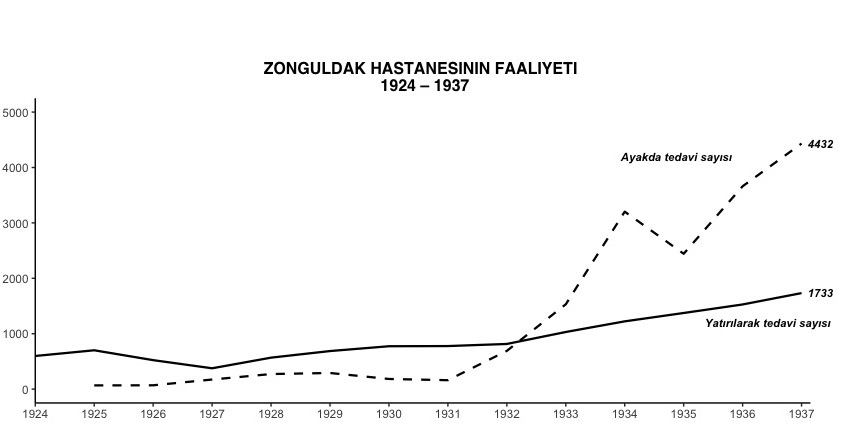
\includegraphics[width=12cm,height=15cm,keepaspectratio]{zonguldak_reinterpreted.png}
	\captionof{figure}{\label{fig:mylabelf4reinter} An alternative illustration of "The service of the Zonguldak Government Hospital, 1924-1937" (\protect\tikz[baseline]{\protect\draw[line width=0.5mm] (0,.8ex)--++(1,0) ;} The number of inpatient treatments  \protect\tikz[baseline]{\protect\draw[line width=0.2mm,densely dashed] (0,.8ex)--++(1,0);} The number of outpatient treatments).}
\end{figure}


Another example can be the Figure~\ref{fig:mylabelf12org}, where the amount of four different drugs, namely, Arsenobenzol, Bizmopen, Mercury, and Iodine, sent by the Department of Control of Syphilis to cities for treatment is displayed. In Figure~\ref{fig:mylabelf12org}, it is easy to compare the amount of four different drugs to each other for a given year. This design choice eliminates  the ability to investigate trends in the amount of a specific drug supplied over the years. To investigate the relationship between and within the drug categories, we can prefer  displaying the amount of each drug over the years separately through faceting with \code{facet\_wrap()} layer.

Figure~\ref{fig:mylabelf12reinter} gives the amount of Arsenobenzol, Bizmopen, Mercury, and Iodine, sent by the Department of Control of Syphilis as a facet line plot, where each sub-panel refers to an individual drug category. We can differentiate the drug categories via stripe titles.  Each sub-panel now
sits on a common horizontal axis, that's years from 1925 to 1937, and a common vertical axis changing from to 0 to the largest possible value in the overall data. Hence, we can clearly and fairly investigate the trend of each drug over the years, and compare drug amounts for a given year. Faceting also enables us to avoid hatching and using legends, resulting in a decrease in the computational burden to implement this figure such that the amount of lines required to code new figure decreased from 101 lines (4520 characters) to 34 lines 
(1441 characters) (please have a look at the \code{R} codes  in the Supplementary material to implement Figures~\ref{fig:mylabelf12} and \ref{fig:mylabelf12reinter}).



\begin{figure}[hbt!]
	\centering
	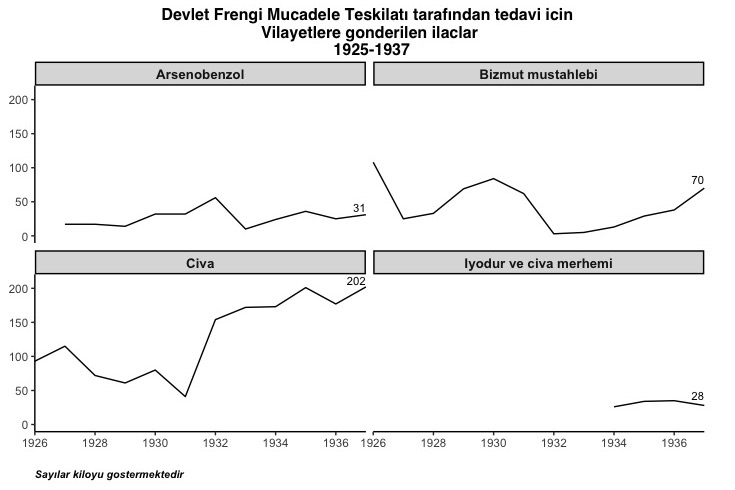
\includegraphics[width=12cm,height=12cm,keepaspectratio]{frengi_reinterpreted.png}
	\captionof{figure}{\label{fig:mylabelf12reinter} An alternative illustration of "The drugs sent by the Department of Control of Syphilis to cities for treatment, 1926-1937" (The upper-left panel is Arsenobenzol, the upper-right panel is Bizmopen, the lower-left panel is Mercury, and the lower-rightpanel is Iodine).}
\end{figure}



Lastly, Figure~\ref{fig:mylabelf14org} shows the service of birth and childcare houses between the years 1926  and 1937. 
The inpatient and the outpatient services are further divided into two categories: Child and Woman. The original design of the graph resembles a population pyramid with the help of creating an illusion that the left-panel (for inpatient services) and  the right-panel (for outpatient services) are symmetric to each other over the vertical axis, when they are not. Indeed, while  the left horizontal axis spans from 0 to 5000, the right horizontal axis  from 0 to 50000 with linear increments. Eliminating 0 strings from horizontal axis labels also contributes this confusion. In the end, as we discussed earlier, this perceptional illusion results in an aesthetically pleasing, but misleading graph. On the other hand, since left and right panels do not share a common horizontal axis, faceting will not result in a fair comparison between panels as done in Figure~\ref{fig:mylabelf12reinter}. Alternatively, Figure~\ref{fig:mylabelf14org} can be split into two sub-line plots with the same horizontal axis, that's the years from 1926 to 1937, and with different vertical axis giving the relative frequencies for inpatient services and outpatient services, respectively. This leads to the Figure~\ref{fig:mylabelf14reinter} which gives more realistic comparison between child and women in terms of inpatient and outpatient services received. Lastly, the amount of lines required to code new figure decreased from 80 lines (3578 characters) to 55 lines 
(2150 characters) (please have a look at the \code{R} codes  in the supplementary material to implement Figures~\ref{fig:mylabelf14} and \ref{fig:mylabelf14reinter}).

For a detailed discussion on effectiveness of graphics, chart design, perception and cognition, we kindly invite readers to read \cite{cleveland1986experiment} and \cite{vanderplas2020testing}.

\begin{figure}[hbt!]
	\centering
	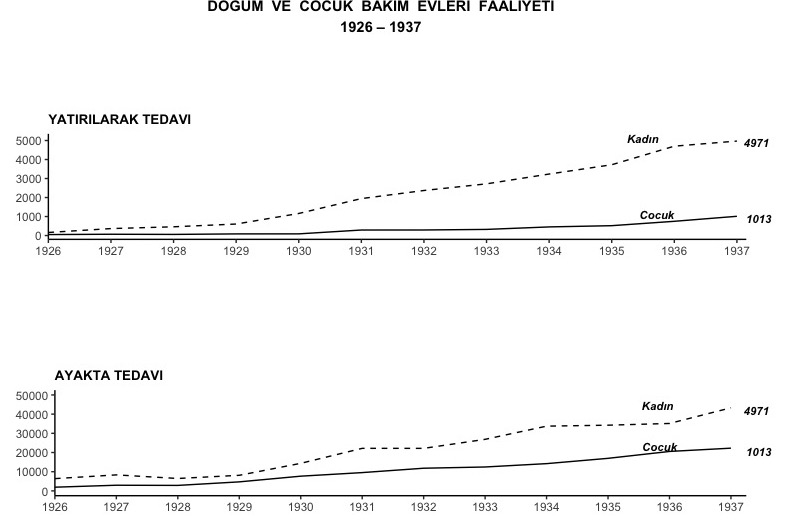
\includegraphics[width=12cm,height=25cm,keepaspectratio]{dogum_reinterpreted.png}
	\captionof{figure}{\label{fig:mylabelf14reinter} An alternative illustration of "The service of birth and childcare houses, 1926-1937" (The upper-panel is for inpatient services and the right-panel is for outpatient services; \protect\tikz[baseline]{\protect\draw[line width=0.5mm] (0,.8ex)--++(1,0) ;} Child  \protect\tikz[baseline]{\protect\draw[line width=0.2mm,densely dashed] (0,.8ex)--++(1,0);} Woman).}
\end{figure}


\section{Conclusion}
\label{sec:conc}

In this study, our aim was two-fold: first understanding the information design behind the historical column bar graphics drawn with hand and published in late $1930$'s, and then, if possible, reproducing these graphics with the help of the advances in data visualization technologies in our era, namely, through \pkg{ggplot2} package. 

While we were dealing with these historical graphics to reproduce them in \pkg{ggplot2} package, we were mostly challanged with  i) multi-line titles with different font styles, ii) textured patterns, and iii) data groups where the difference of the frequencies is not monotonic over the years. 

In a multi-line title or any multi-line text within a figure plotting area such as tick mark labels, data labels, legends, and so on, if interest is on changing font face i.e., making text bold or italic, then simple  \code{Markdown} syntax would be integrated into text and rendered with the help of  \code{element\_markdown()} layer in the \CRANpkg{ggtext} package \citep{ggtext}. However, if more aesthetic changes such as font family type, size, or color are needed in the text, then the text can be manipulated appropriately with the corresponding \code{HTML} tags, and rendered with \code{element\_textbox()} layer in the \pkg{ggtext} package. We also provided  \code{R} codes to produce the multi-lines in the Figure~\ref{fig:mylabelf1org} and ~\ref{fig:mylabelf12org} in the supplementary material. 

On the other hand, \CRANpkg{ggpattern} package \citep{pattern} provides geometric based patterns such as stripe, crosshatch,  or circle to \code{ggplot2 }objects with \code{geom\_col\_pattern()} layer. If a specific pattern is required in bars, then  \code{geom\_pattern\_manual()} layer enables to assign the desired pattern to a specific bar. This order is reflected into the legend keys as well. For comparison,  we reproduced the Figure~\ref{fig:mylabelf12}  with \pkg{ggpattern} and presented it in Figure~\ref{fig:mylabelf12pat}. The amount of lines to produce Figure~\ref{fig:mylabelf12pat}  is now 51 (2171 characters), where 
\code{R} codes are available in the supplementary material. 

Unfortunately, the last challenge requires more work which can be considered as a future study.

\begin{figure}[hbt!]
	\centering
	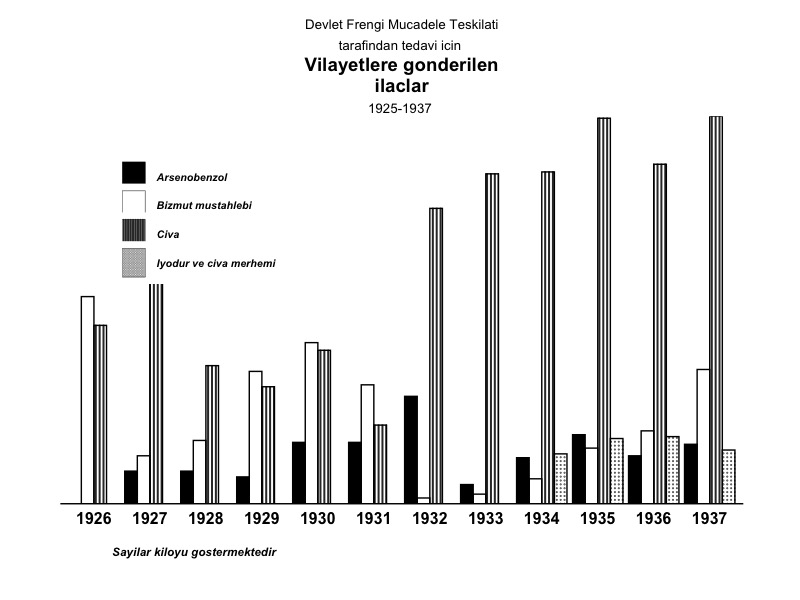
\includegraphics[width=13cm,height=18cm,keepaspectratio]{frengi_ggpattern.png}
	\captionof{figure}{\label{fig:mylabelf12pat} An alternative illustration of "The drugs sent by the Department of Control of Syphilis to cities for treatment, 1926-1937"  ($\blacksquare$ Arsenobenzol  $\square$ Bizmopen  \crule[gray]{0.30cm}{0.30cm} (textured pattern with vertical lines)  Mercury \legendsquare{pattern=dots}~Iodine).}
\end{figure}


In today's Covid-19 pandemic, we also saw that data visualization helped us to better understand the Covid-19 related statistics, i.e., the number of confirmed cases, the number of recovered cases, the number of active cases, and the number of deaths. It can be said that John Burn-Murdoch’s Financial Times charts played a leading role in the visualization of Covid-19 related statistics through line charts. With the help of today's technological advances in data visualization, many other media outlets such as New York Times and the Guardian take advantage of zoomable and scrollable graphics for visually attractive story telling. Furthermore, unlike the past, GIS-based interactive data visualization examples such as CNN health's Covid-19 tracker \citep{CNN} came into play for spatially investigating the progress of the disease and/or vaccination. Nevertheless, understanding all these visualizations from the viewer's side requires data literacy.

What we experienced during the Covid-19 pandemic also enabled us to better understand the historical graphics used in our study. When we were dealing with these graphics back in late $2019$, it was our limited understanding of how important the workload and capacity of hospitals was during an epidemic or a pandemic and how important the services of government, private, and mobile hospitals were for carrying the workload in the fight against the infectious diseases in order to \enquote{flatten the curve}. Furthermore, we also learned that, as in the Figure~\ref{fig:mylabelf7}, while epidemics take a very long time to be diminished from the world and even if the ratio of \enquote{the number of blood tests} to \enquote{the number of positive test results} is getting larger over the years, increasing the test capacity was also an old school approach yielding the idea \enquote{The more tests the better prevention is}. 

Lastly, we can conclude that neither pandemics, nor the data visualization is new to our world. As in the past and today, statistical graphics and data visualization play a vital bridge role between the authorities and the public during global issues such as health.






%\newpage
%\clearpage

\section*{Acknowledgment}
We would like to thank Assoc. Prof. Dr. Eminalp Malkoc from Department of History at Istanbul Technical University for providing us the original statistical graphics used in this paper. We would also like
to thank the reviewer whose comments improved the quality of the paper.



\bibliography{inan}

\address{Sami Aldag\\
Department of Mathematics Engineering, \\
Istanbul Technical University, \\
Istanbul, 34469,\\
Turkey \\
 % (ORCiD if desired)\\
  \email{aldag@itu.edu.tr}}

\address{Dogukan Topcuoglu\\
Department of Mathematics Engineering, \\
Istanbul Technical University, \\
Istanbul, 34469,\\
Turkey \\
 \email{topcuoglud@itu.edu.tr}}

\address{Gul Inan\\
Department of Mathematics, \\
Istanbul Technical University, \\
Istanbul, 34469,\\
Turkey \\
 (ORCiD: 0000-0002-3981-9211)\\
  \email{inan@itu.edu.tr}}
